\section{Introduction}

\section{Decision Trees}

Decision trees can be used for both regression and classification. They provide
the foundation for the tree-based models considered in this work, with particular
emphasis on regression trees\footnote{A regression tree is a particular type of
decision tree designed for regression problems.}. The construction of a tree is
based on the recursive partitioning of the predictor space, where each partition
defines a node and the final resulting partitions are referred to as leaves or
terminal nodes. At each internal node, a splitting condition is defined based on
one or more predictors. If the condition is satisfied, the observation is directed
to one of the resulting child nodes; otherwise, it is directed to the other child
node. This process is repeated recursively until the terminal nodes are reached.
An example of a regression tree is presented in Figure~\ref{fig:fig-arvore}.

\begin{figure}[htb]
    \centering
    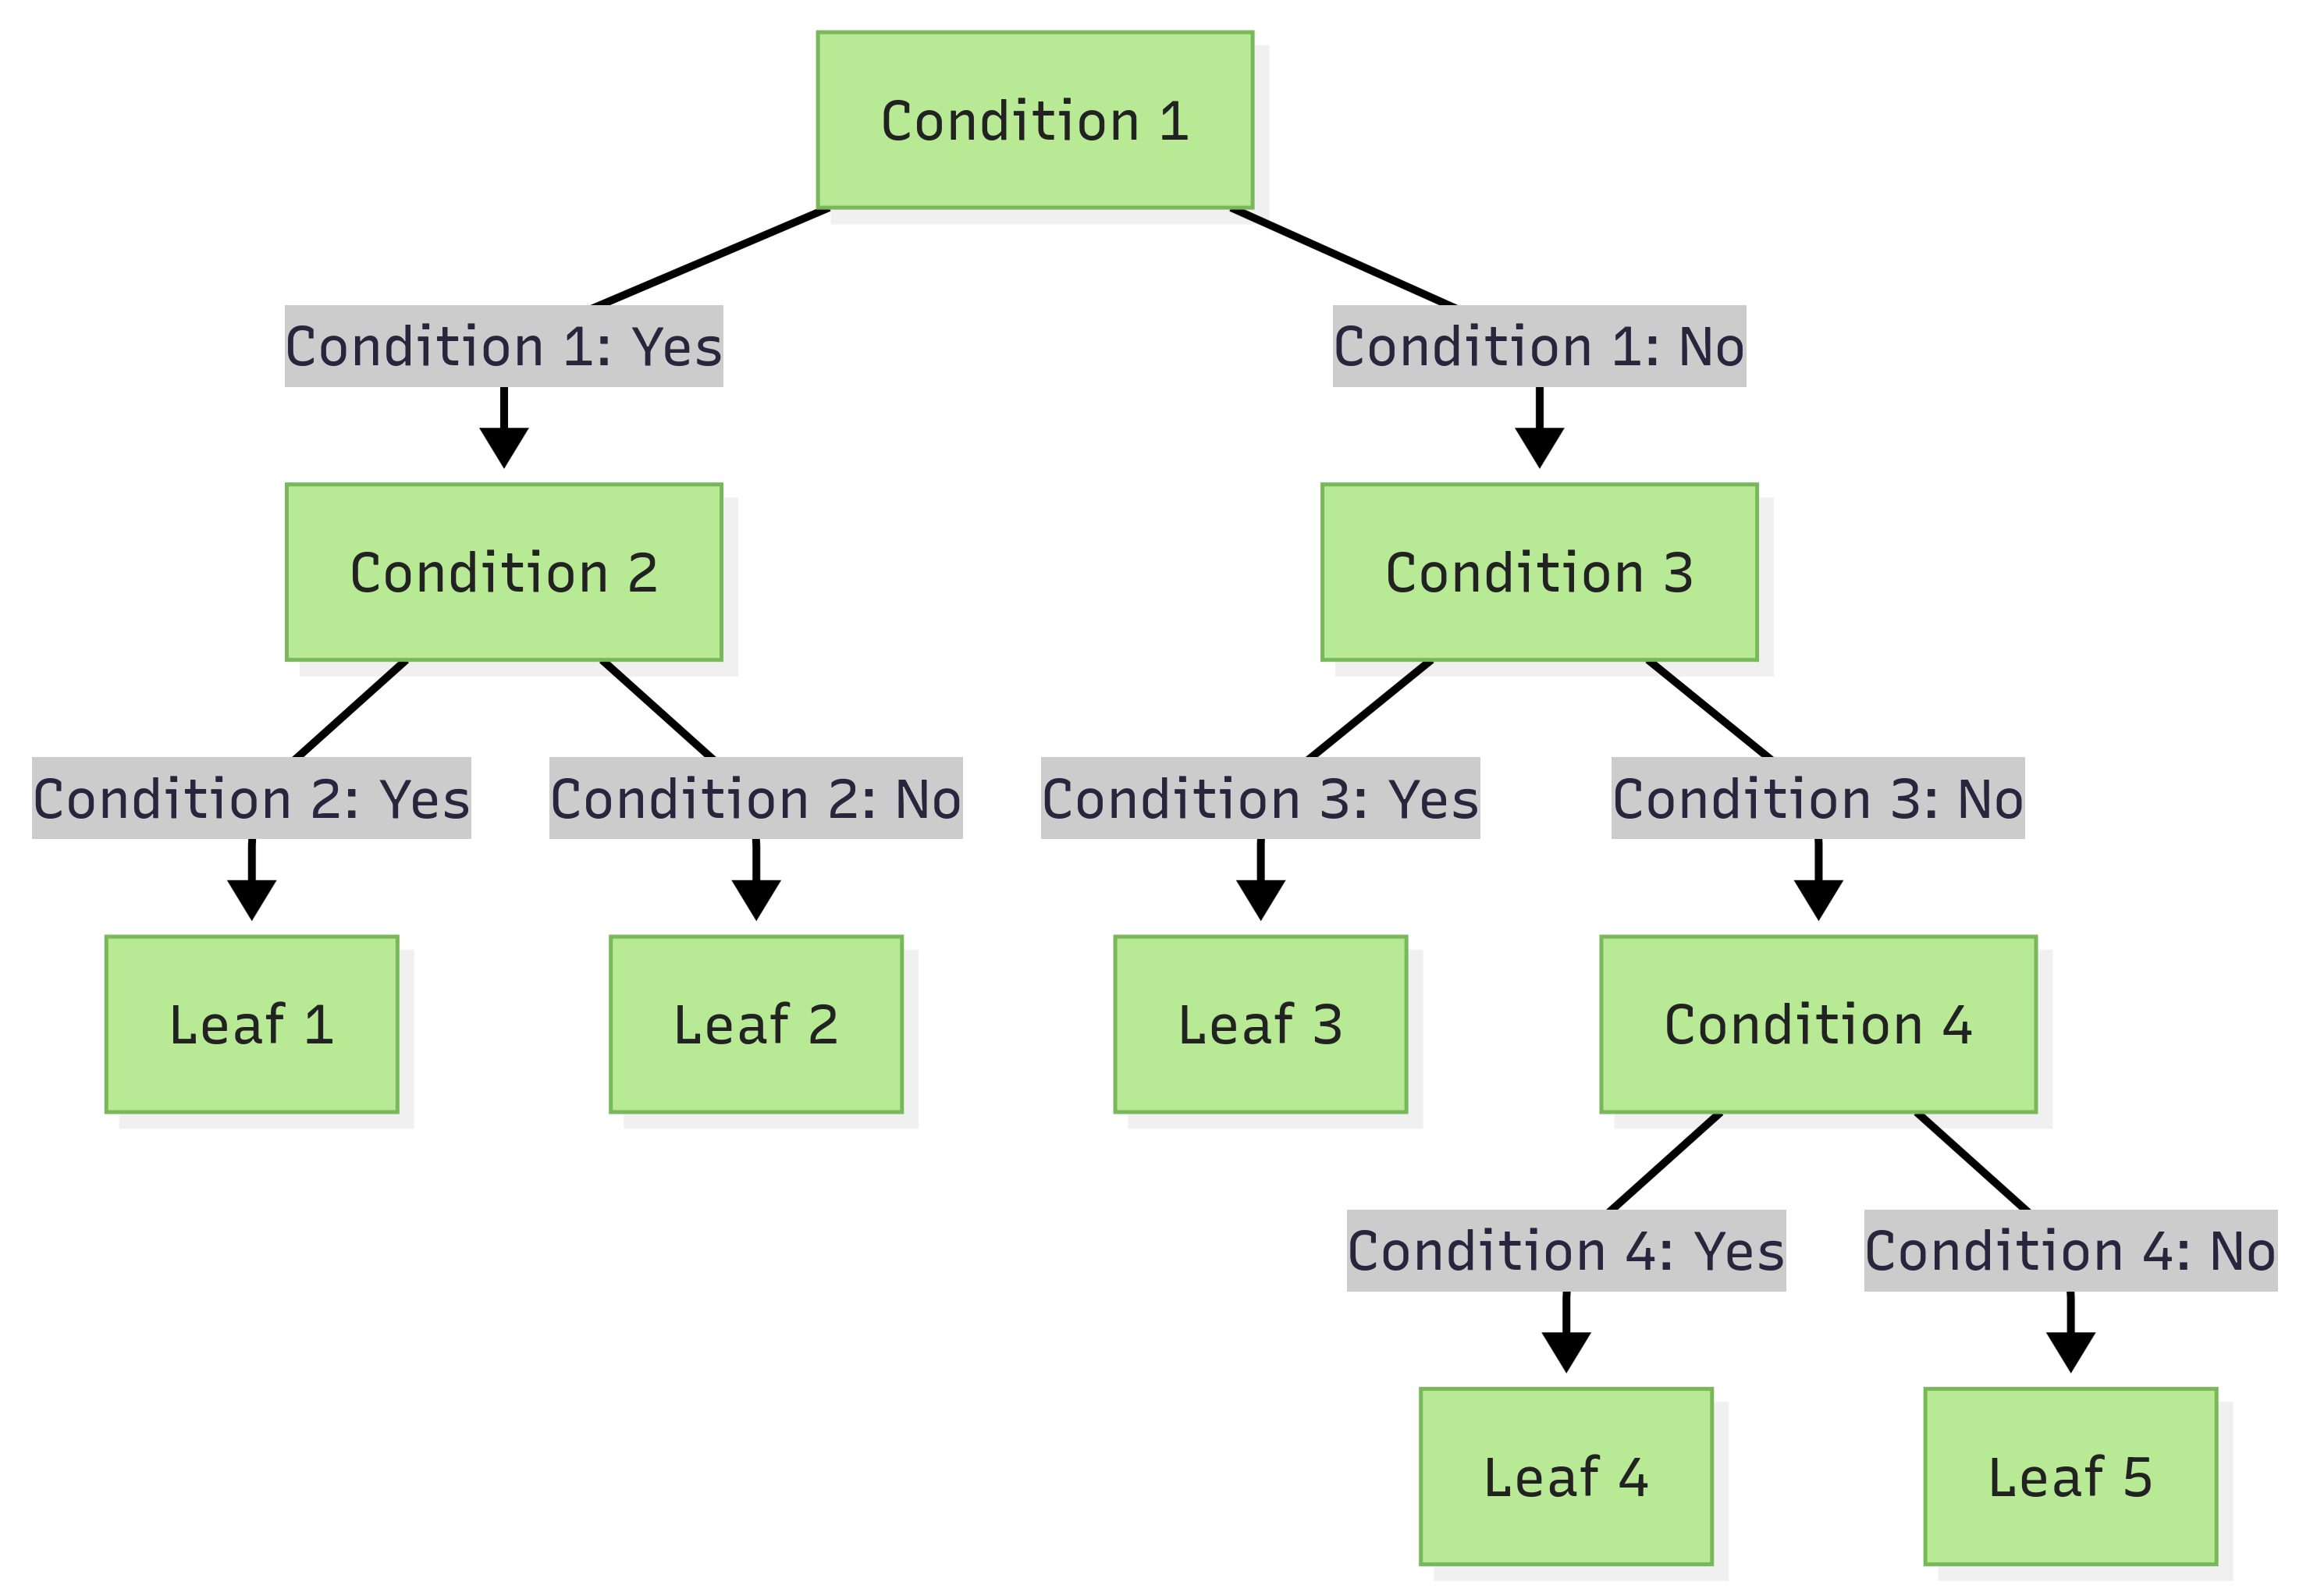
\includegraphics[width=0.8\textwidth]{images/mermaid-tree.png}
    \caption{Example of a regression tree. The tree has five terminal nodes and
    four internal nodes.}
    \label{fig:fig-arvore}
\end{figure}

For a regression problem, the predictor space is partitioned into $J$ distinct
and disjoint regions, denoted by $R_1, R_2, \ldots, R_J$. These regions are
typically constructed as rectangular or box-shaped regions through recursive
binary splitting, with the objective of minimizing the residual sum of squares.
The response variable can then be modeled as a constant $c_j$ within each region
$R_j$. Thus, the resulting regression tree can be represented by
\begin{equation}
\label{eq:regression_tree}
f\left(x\right)
=
\sum_{j=1}^{J} c_j I\left(x \in R_j\right)\text{.}
\end{equation}

The estimator of the constant $c_j$ is obtained by the method of least
squares. Thus, for a given region $R_j$, $c_j$ is chosen to minimize $\sum_{x_i \in R_j} \left[y_i - f\left(x_i\right)\right]^2$.
Since $x_i \in R_j$, the indicator function associated with $R_j$ satisfies
\begin{equation}
I_{R_j}(x_i) =
\begin{cases}
    1, & \text{if } x_i \in R_j,\\
    0, & \text{if } x_i \notin R_j.
\end{cases}
\end{equation}

Because the regions are disjoint, each observation belongs to at most one
region. Therefore, for $x_i \in R_j$, the representation in
Equation~\eqref{eq:regression_tree} reduces to $f\left(x_i\right) = c_j$.
Consequently, the least-squares problem within region $R_j$ reduces to
minimizing
\begin{equation}
\sum_{x_i \in R_j} \left(y_i-c_j\right)^2
\end{equation}
with respect to $c_j$. Differentiating with respect to $c_j$ gives
\begin{equation}
\label{eq:partialdev}
\frac{\partial}{\partial c_j}
\sum_{x_i \in R_j} \left(y_i-c_j\right)^2
=
-2\sum_{x_i \in R_j}\left(y_i-c_j\right).
\end{equation}
Setting Equation~\eqref{eq:partialdev} equal to zero yields
\begin{equation}
\sum_{x_i \in R_j}
\left(y_i-\hat{c}_j\right)=0.
\end{equation}

Expanding the summation and denoting by $N_j$ the number of observations
in region $R_j$, it follows that the estimator of $c_j$, denoted by
$\hat{c}_j$, is simply the sample mean of the observed responses $y_i$
within $R_j$:
\begin{equation}
\label{eq:estimacjdev}
\sum_{x_i \in R_j} y_i - \hat{c}_j N_j = 0
\quad\Rightarrow\quad
\hat{c}_j =
\frac{1}{N_j}\sum_{x_i \in R_j} y_i.
\end{equation}

However, as noted by \citeonline{james2021introduction}, considering all
possible partitions of the predictor space into $J$ regions is
computationally infeasible due to the large number of possible
partitions. Therefore, a recursive binary splitting procedure is adopted.
The process begins at the root node, which contains all observations, and
successively partitions the predictor space into increasingly smaller
regions. Each split produces two child nodes, as illustrated in
Figure~\ref{fig:fig-arvore}.

To perform recursive binary splitting, one first selects a predictor
$X_j$ and a cutpoint $s$ such that the resulting partition produces the
largest possible reduction in the residual sum of squares. For a given
predictor and cutpoint, the predictor space is divided into the two
regions
\begin{equation}
R_{1}(j,s) = \{x : x_j \leq s\}
\quad\text{and}\quad
R_{2}(j,s) = \{x : x_j > s\}.
\end{equation}
The predictor $j$ and cutpoint $s$ are then selected by solving
\begin{equation}
\min_{j,s}
\left[
\min_{c_1}
\sum_{x_i \in R_1(j,s)}
\left(y_i-c_1\right)^2
+
\min_{c_2}
\sum_{x_i \in R_2(j,s)}
\left(y_i-c_2\right)^2
\right],
\end{equation}
where $c_1$ and $c_2$ are the mean responses in the regions
$R_1(j,s)$ and $R_2(j,s)$, respectively. Once the optimal split is
determined, the observations are partitioned into the two resulting
regions, and the same procedure is recursively applied to each
subregion.

The size of a regression tree controls the complexity of the resulting
model. An excessively large tree may overfit the training data by capturing
not only relevant patterns but also random noise. Consequently, although
such a model may achieve low prediction error on the training data, its
performance on new observations may deteriorate due to poor generalization.
Conversely, a tree that is too small may fail to capture important patterns
and relationships present in the data. A common strategy for controlling
tree complexity is therefore to first grow a large tree $T_0$, stopping the
splitting process only when a specified minimum number of observations is
reached in each terminal node. The resulting tree is then pruned according
to the cost-complexity criterion, defined below.

Consider a tree $T$ obtained by pruning $T_0$, such that $T \subseteq T_0$.
Let $N_j$ denote the number of observations in region $R_j$. The residual
sum of squares within region $R_j$ can be expressed in terms of the
mean squared error
\begin{equation}
Q_j(T)
=
\frac{1}{N_j}
\sum_{x_i \in R_j}
\left(y_i-\hat{c}_j\right)^2.
\end{equation}
The cost-complexity criterion is then defined as
\begin{equation}
C_{\alpha}(T)
=
\sum_{j=1}^{|T|}
N_j Q_j(T)
+
\alpha |T|,
\end{equation}
where $|T|$ denotes the number of terminal nodes of the tree and
$\alpha\geq0$ is a complexity parameter that controls the trade-off between
the goodness of fit and the size of the tree. For each value of $\alpha$,
the optimal subtree is defined as
\begin{equation}
T_{\alpha}
=
\underset{T\subseteq T_0}{\operatorname{argmin}}
\; C_{\alpha}(T).
\end{equation}
Larger values of $\alpha$ impose a greater penalty on tree complexity and
therefore favor smaller trees, whereas smaller values of $\alpha$ favor
larger trees. When $\alpha=0$, the complexity penalty vanishes and the
resulting tree is $T_0$.

The sequence of subtrees can be obtained through a weakest-link pruning
procedure, in which internal nodes are successively collapsed according
to the increase in the residual sum of squares per terminal node removed.
This procedure produces a finite sequence of nested subtrees, from which
the optimal tree can be selected for a given value of $\alpha$.

The complexity parameter $\alpha$ can be selected using $K$-fold cross-
validation, commonly with $K=5$ or $K=10$. The final regression tree is
then given by $T_{\hat{\alpha}}$. The overall procedure for constructing
and pruning a regression tree is summarized in
Algorithm~\ref{alg:algo-buildtree}.

\begin{algorithm}[H]
\caption{Construction and pruning of a regression tree
\cite{james2021introduction}.}
\label{alg:algo-buildtree}
\begin{algorithmic}[1]

\State \textbf{1.} Use recursive binary splitting to grow a large tree
$T_0$ on the training data, stopping only when each terminal node
contains fewer than a specified minimum number of observations.

\State \textbf{2.} Apply the cost-complexity criterion to $T_0$ to obtain
a sequence of optimal subtrees $T_{\alpha}$ for different values of
$\alpha$.

\State \textbf{3.} Use $K$-fold cross-validation to select $\alpha$.
Partition the training observations into $K$ folds. For each
$k=1,\ldots,K$:

\State \hspace{1em} (a) Repeat Steps 1 and 2 using all folds except the
$k$-th fold.

\State \hspace{1em} (b) Evaluate the mean squared prediction error on the
held-out $k$-th fold for each candidate value of $\alpha$.

\State \hspace{1em} Average the validation errors across the $K$ folds for
each value of $\alpha$, and select $\hat{\alpha}$ that minimizes the
average error.

\State \textbf{4.} Return the subtree $T_{\hat{\alpha}}$ corresponding to
the selected value $\hat{\alpha}$.

\end{algorithmic}
\end{algorithm}

For classification trees, the main differences from regression trees lie
in the criterion used to evaluate node splits and in the way predictions
are assigned to terminal nodes. For a classification tree, consider a node
$j$ corresponding to a region $R_j$ containing $N_j$ observations. The
predicted class is typically the majority class within that node. The
proportion of observations belonging to class $k$ is given by
\begin{equation}
\hat{p}_{jk}
=
\frac{1}{N_j}
\sum_{x_i \in R_j}
I\left(y_i=k\right).
\end{equation}
Thus, each observation in node $j$ is assigned to the class
\begin{equation}
k(j)
=
\underset{k}{\operatorname{argmax}}\;\hat{p}_{jk},
\end{equation}
corresponding to the class with the largest estimated proportion in that
node.

While the residual sum of squares is used as the impurity measure for
regression trees, several measures can be used for classification trees.
Common choices include the classification error rate, the Gini index, and
cross-entropy. These measures quantify the degree of
heterogeneity among the classes within a node and are used to evaluate
candidate splits.

\section{Ensemble Methods}

Decision trees offer an interpretable and flexible approach to predictive
modeling. However, individual trees can be sensitive to variations in the
training data, leading to substantial variability in their predictions.
Ensemble learning provides a general framework for addressing this
limitation by combining multiple base learners into a single predictive
model.

According to \citeonline{hastie2009elements}, ensemble methods can be viewed
as involving two main steps. First, a collection of base learners is
constructed from the training data, potentially using different samples,
features, or learning procedures. Second, the predictions from these
learners are combined to produce an aggregate estimator. The resulting
model can achieve improved predictive performance and stability relative
to individual base learners. The following sections describe the ensemble methods
considered in this work.


\subsection{Bagging}

Bootstrap aggregation, commonly referred to as Bagging, was introduced by
\citeonline{breiman1996bagging}. Its main idea is to construct an aggregate
estimator by fitting multiple versions of a base learner to bootstrap
samples drawn from the training data. The predictions from these learners
are subsequently combined to obtain the final prediction. By averaging
multiple fitted models, Bagging can reduce the variance of unstable
learning algorithms and consequently improve the stability and predictive
performance of the resulting model. In particular, Bagging can be applied
to regression trees to mitigate the high variability associated with
individual trees.

More formally, let $\mathcal{L}$ denote the training set and let
$\{\mathcal{L}^{\left(i\right)}\}^{B}_{i=1}$ denote $B$ bootstrap samples
drawn independently from $\mathcal{L}$. For each bootstrap sample, a base
learner $f$ is fitted, resulting in the collection $f\left(x,\mathcal{L}^{(1)}\right),\ldots, f\left(x,\mathcal{L}^{(B)}\right)$.
When the response variable $y$ is continuous, the Bagging estimator is
obtained by averaging the predictions across the $B$ fitted models:
\begin{equation}
\label{eq:bagging_regression}
f_B(x)
=
\frac{1}{B}
\sum_{b=1}^{B}
f\left(x,\mathcal{L}^{(b)}\right).
\end{equation}
Here, $f_B(x)$ denotes the aggregated prediction at $x$.

For classification problems, the predictions are instead combined through majority voting. Let the possible classes be indexed by
$j\in\{1,\ldots,J\}$, and define
\begin{equation}
N_j(x) = \sum_{b=1}^{B} I\left\{ f\left(x,\mathcal{L}^{(b)}\right)=j \right\}\text{,}
\end{equation}
where $N_j(x)$ denotes the number of bootstrap models that assign
observation $x$ to class $j$. The Bagging classification rule is then
given by
\begin{equation}
\label{eq:bagging_classification}
f_B(x)
=
\underset{j\in\{1,\ldots,J\}}{\operatorname{argmax}}
\;N_j(x).
\end{equation}
Thus, the predicted class is the one receiving the largest number of votes
among the $B$ fitted base learners.


\section{Gradient Boost}

\section{Kernel Methods}

\noindent Kernel-based methods are highly flexible techniques that can be used
to extend models or algorithms to nonlinear decision regions \cite{mohri2018foundations}.
These methods are based on kernel functions, which, under symmetry and
positive semidefiniteness conditions, can be interpreted as inner products
in high-dimensional feature spaces. In particular, positive semidefinite
kernels are associated with Reproducing Kernel Hilbert Spaces (RKHS).
Therefore, this section aims to introduce the fundamental concepts of
kernel-based methods, including the definition of kernel functions, positive
semidefinite kernels, the representer theorem, and Reproducing Kernel Hilbert
Spaces (RKHS).

\section{Kernels}

By definition, a function $K: \mathcal{X} \times \mathcal{X} \to \mathbb{R}$
is called a kernel on $\mathcal{X}$. A central idea is to construct a kernel
$K$ such that, for any two points $x, x' \in \mathcal{X}$,
$K(x,x')$ corresponds to the inner product between representations of these
points in a Hilbert space $\mathcal{H}$, that is,
\begin{equation}
\forall x, x' \in \mathcal{X}, \quad
K(x,x') = \langle \phi(x), \phi(x') \rangle_{\mathcal{H}},
\end{equation}
for some mapping $\phi: \mathcal{X} \to \mathcal{H}$. The space
$\mathcal{H}$ is referred to as the feature space.

From this perspective, the kernel can be interpreted as a measure of
similarity between elements of $\mathcal{X}$, since the inner product
provides a notion of similarity between their representations in the
feature space.

A fundamental advantage of this approach is computational. In many cases,
it is significantly more efficient to compute $K(x,x')$ directly than to
explicitly compute $\phi(x)$ and $\phi(x')$ and then evaluate their inner
product. This idea is commonly referred to as the \textit{kernel trick}.

\subsection{Positive Semidefinite Kernels}

For a function $K$ to be used as a positive semidefinite kernel, it must
satisfy the appropriate symmetry and positive semidefiniteness conditions.
These properties allow the kernel to induce a consistent inner-product
structure and, consequently, a geometry in a suitable Hilbert space.

Formally, a kernel $K: \mathcal{X} \times \mathcal{X} \to \mathbb{R}$ is
said to be positive semidefinite if, for any finite set
$\{x_1, \ldots, x_n\} \subset \mathcal{X}$, the Gram matrix
\begin{equation}
\mathbf{K} = [K(x_i,x_j)]_{i,j=1}^n
\in \mathbb{R}^{n \times n}
\end{equation}
is positive semidefinite. That is, for any vector
$\mathbf{c}=(c_1,\ldots,c_n)^\top \in \mathbb{R}^n$,
\begin{equation}
\mathbf{c}^\top \mathbf{K}\mathbf{c}
=
\sum_{i=1}^n \sum_{j=1}^n
c_i c_j K(x_i,x_j)
\geq 0.
\end{equation}

Equivalently, all eigenvalues of $\mathbf{K}$ are nonnegative. This
property is essential because it guarantees that the kernel admits a
consistent inner-product representation in a Hilbert space.
\subsection{Hilbert Spaces}

The notion of a Hilbert space provides the mathematical structure required
for the theory of kernels.

By definition, a Hilbert space $\mathcal{H}$ is a vector space equipped with
an inner product $\langle \cdot, \cdot \rangle_{\mathcal{H}}$ that is complete
with respect to the norm induced by this inner product. The norm on
$\mathcal{H}$ is defined by
\begin{equation}
\forall h \in \mathcal{H}, \quad
\|h\|_{\mathcal{H}}
=
\sqrt{\langle h,h\rangle_{\mathcal{H}}}.
\end{equation}

Completeness implies that every Cauchy sequence in $\mathcal{H}$ converges
to an element that also belongs to $\mathcal{H}$. This property is important
in approximation and optimization problems, as it ensures that limits of
convergent sequences remain within the space.

In the context of kernel methods, the Hilbert space provides the space in
which data can be represented through a feature mapping $\phi$.

\subsection{Reproducing Kernel Hilbert Spaces}

The relationship between positive semidefinite kernels and Hilbert spaces
can be formalized through the theory of Reproducing Kernel Hilbert Spaces
(RKHS).

Let $K: \mathcal{X} \times \mathcal{X} \to \mathbb{R}$ be a symmetric
positive semidefinite kernel. Then, there exists a Hilbert space
$\mathcal{H}$ of functions on $\mathcal{X}$ such that, for every
$x,x' \in \mathcal{X}$,
\begin{equation}
K(x,x')
=
\langle K(x,\cdot), K(x',\cdot) \rangle_{\mathcal{H}}.
\end{equation}

Moreover, $\mathcal{H}$ satisfies the so-called reproducing property:
\begin{equation}
\forall h \in \mathcal{H}, \forall x \in \mathcal{X}, \quad
h(x)
=
\langle h, K(x,\cdot)\rangle_{\mathcal{H}}.
\end{equation}

The reproducing property implies that the evaluation functional
$h \mapsto h(x)$ is continuous for every $x \in \mathcal{X}$ and can be
represented by the function $K(x,\cdot)$ through the Riesz representation
theorem.

A Hilbert space satisfying these properties is called a Reproducing Kernel
Hilbert Space (RKHS) associated with the kernel $K$. RKHSs play a central
role in statistical learning methods, particularly in regularization,
nonparametric estimation, and supervised learning.

\subsection{Representer Theorem}

One of the most important results for the formulation of the GG-KM model
is the Representer Theorem. Its main importance lies in the fact that,
although the optimization is performed over a potentially infinite-dimensional
space, an optimal solution can be expressed as a finite linear combination
of kernels evaluated at the observations in the sample.

Formally, let $K : \mathcal{X} \times \mathcal{X} \to \mathbb{R}$ be a
positive semidefinite kernel and let $\mathcal{H}$ be its associated RKHS.
For any nondecreasing function $G : \mathbb{R} \to \mathbb{R}$ and any loss
function $L : \mathbb{R}^n \to \mathbb{R} \cup \{+\infty\}$, consider the
optimization problem
\begin{equation}
\min_{h \in \mathcal{H}}
\left\{
G\left(\|h\|_{\mathcal{H}}\right)
+
L\left(h(x_1),\ldots,h(x_n)\right)
\right\}.
\end{equation}
Under the appropriate conditions for the existence of a minimizer, this
problem admits a solution of the form
\begin{equation}
h^{*}(\cdot)
=
\sum_{i=1}^{n}\alpha_i K(x_i,\cdot).
\end{equation}
If $G$ is strictly increasing, then every minimizer admits this
representation.

This result is particularly relevant because it reduces a functional
optimization problem in an infinite-dimensional space to a finite-dimensional
optimization problem involving only the coefficients
$\boldsymbol{\alpha}=(\alpha_1,\ldots,\alpha_n)^\top$. In practice, this
makes kernel-based methods computationally feasible and shows that the
necessary information for estimation can be obtained from the kernel matrix,
without explicitly computing the feature mapping $\phi(\cdot)$.

% The choice of kernel implicitly determines the class of functions contained
% in the associated RKHS and, consequently, the complexity of the functions
% that the model can represent. In this context, the kernel and its associated
% parameters, such as $\gamma$, $d$, and $\sigma$, can be regarded as
% hyperparameters controlling the complexity of the model.
